% -------------------------------------------------------------------------------------------------
%
%  Skeleton for Control Systems I project at the Institute for Dynamic Systems and Control
% -------------------------------------------------------------------------------------------------
%
% FILENAME:   thesis.tex
%
% ABSTRACT:   main file for theses
%
% EXCEPTIONS: -
%
% USAGE:      !!!!!!COMPILE WITH PDFLATEX, *NOT* WITH LATEX OR TEX!!!!!!!
%
% HISTORY:    written by Sascha A. Stoeter <stoeter@iris.ethz.ch>, www.stoeter.com, 02.06.2004
%             modified by Martin Probst, 18.08.2004
%             modified by Chauncey Graetzel, 11.05.2005
%			  modified by Julian Zilly, 1.12.2017

% -------------------------------------------------------------------------------------------------

\documentclass[12pt,a4paper,twocolumn]{article}
\usepackage{idsc_article}

% -------------------------------------------------------------------------------------------------
% Add needed packages. Some generally useful packages are listed for
% your convenience.
% -------------------------------------------------------------------------------------------------
\usepackage{subfigure}                          % enable the use of subfigures
%\usepackage[bf]{caption}                       % must go after subfigure
\usepackage[thickspace,thinqspace]{SIunits}     %
\usepackage{url}

\usepackage{hyperref}                           % enable Hyperlinks in pdf/ps Docs
\usepackage{enumitem}

% -------------------------------------------------------------------------------------------------
% Some handy definition to simplify future markup changes
% -------------------------------------------------------------------------------------------------
\providecommand{\eg}{e.g.}
\providecommand{\etal}{\textit{et al.}}
\providecommand{\ie}{i.e.}

%\setlength{\textwidth}{18cm} \setlength{\oddsidemargin}{-1cm}
%\setlength{\evensidemargin}{-1cm}

% -------------------------------------------------------------------------------------------------
% Select type of thesis
% -------------------------------------------------------------------------------------------------
\renewcommand{\idscthesistype}{Control Systems I: Seesaw project report}

% -------------------------------------------------------------------------------------------------
% Set names
% -------------------------------------------------------------------------------------------------

% TODO: FILL NAMES HERE
\renewcommand{\idscauthor}{Student name \& Student name \\
Student numbers \\
 XX-XXX-XXX \&  XX-XXX-XXX \\
 email1@ethz.ch \& email2@ethz.ch}



% -------------------------------------------------------------------------------------------------
% Beginning of the main document body
% -------------------------------------------------------------------------------------------------
\begin{document}


% This is the first part of the front matter. Pages appear unnumbered
% and the pages are not counted.

% Title page: set title and date preferably formatted according to
% ISO 8601
\idsctitlepage{Seesaw - Designing a controller}{2017}


% This is the second part of the front matter. Pages appear with
% lowercase roman numbering. The first page number is 'i'.

% List of tab

\pagenumbering{arabic}

\section*{Writing the report}

This text provides some additional hints and examples for the
layout and style of the project report. Your report should no longer than 3 pages including figures. The purpose is both to showcase the work that you have done with the Seesaw as well as to introduce you to writing proper reports in Latex which you yourself still understand years later. 

Delete these introductory paragraphs before submitting your report. Only the sections for the tasks should be submitted. 

\subsection*{Figures}

Figure~\ref{fig:seesaw_task1_fig1} shows a simple figure with a single picture. Please substitute your plots here. Use the caption to describe your figure. A figure should be understandable from the figure alone if possible. 


\subsection*{Miscellaneous}

\begin{description}

\item[Contractions.] Avoid contractions. For instance, use ``do not''
  rather than ``don't.''

\end{description}


\section*{Task 1: Trajectory following}
\label{s:task_1}



\begin{enumerate}[label=\alph*)]
\item Lorem ipsum dolor sit amet, consectetur adipiscing elit, sed do eiusmod tempor incididunt ut labore et dolore magna aliqua. Ut enim ad minim veniam, quis nostrud exercitation ullamco laboris nisi ut aliquip ex ea commodo consequat. 

\item Duis aute irure dolor in reprehenderit in voluptate velit esse cillum dolore eu fugiat nulla pariatur. Excepteur sint occaecat cupidatat non proident, sunt in culpa qui officia deserunt mollit anim id est laborum.
\end{enumerate}

\begin{figure}[ht]
\centering
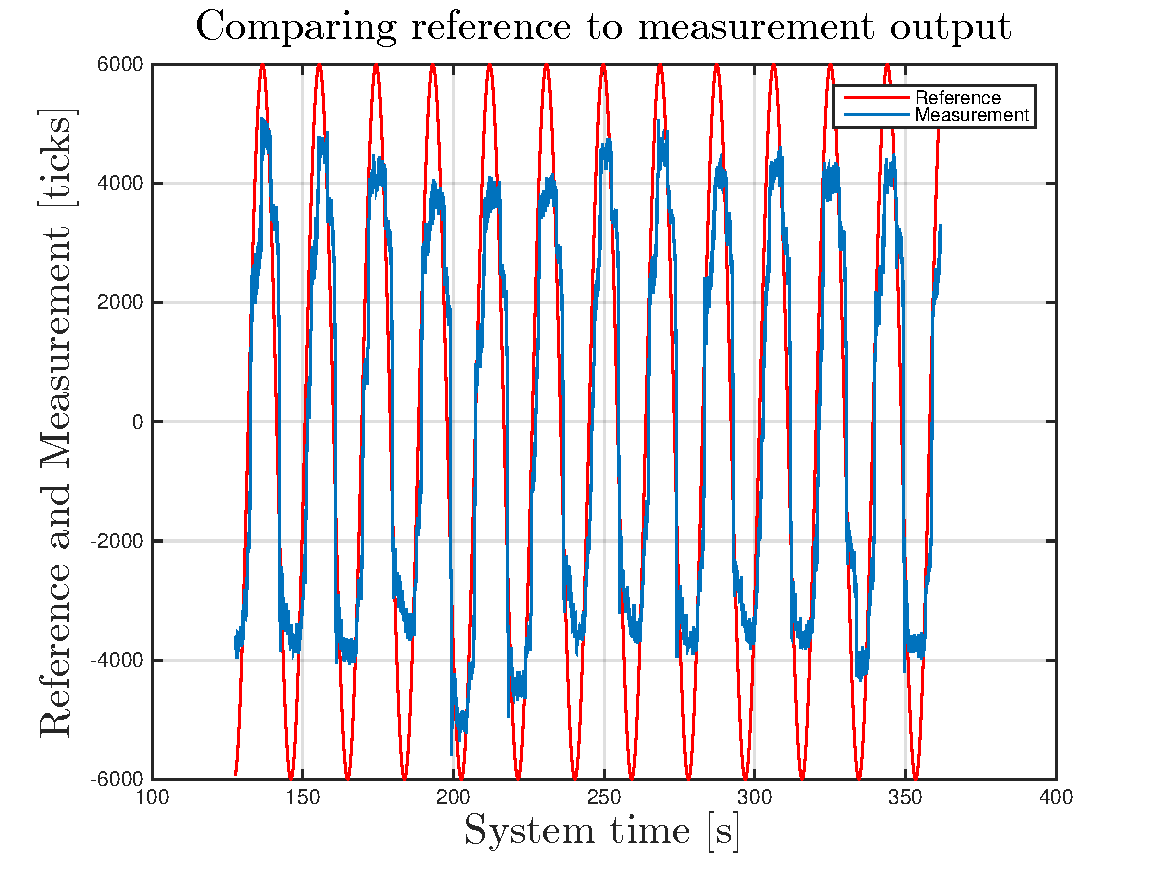
\includegraphics[width=.95\linewidth]{figures/seesaw_measurement_task1_fig1}
\caption[Measure1]{\label{f:measure1} Figure depicting the trajectory following task. The reference trajectory is plotted in red, while the obtained measurements are colored in blue.}
\label{fig:seesaw_task1_fig1}
\end{figure}

\begin{figure}[ht]
\centering
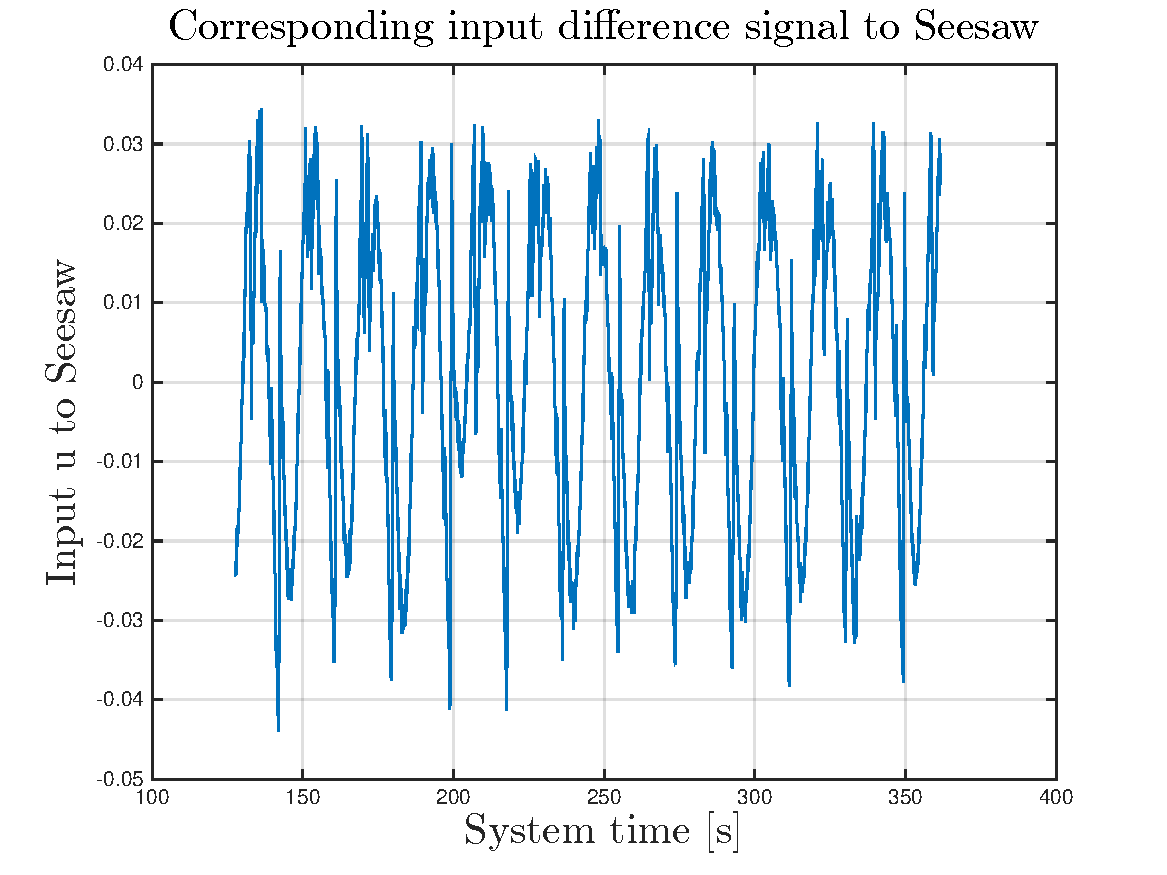
\includegraphics[width=.95\linewidth]{figures/seesaw_measurement_task1_fig2}
\caption[Measure1]{\label{f:measure1} Figure depicting the input command for the trajectory following task to the Seesaw in blue.}
\label{fig:seesaw_task1_fig2}
\end{figure}


\begin{equation*}
\text{Error}_{\text{Task 1}} = \text{FILL IN HERE}
\end{equation*}



\section*{Task 2: Building a controller up to specifications}
\label{s:task_2}

\begin{enumerate}[label=\alph*)]
\item Lorem ipsum dolor sit amet, consectetur adipiscing elit, sed do eiusmod tempor incididunt ut labore et dolore magna aliqua. Ut enim ad minim veniam, quis nostrud exercitation ullamco laboris nisi ut aliquip ex ea commodo consequat. 

\item Duis aute irure dolor in reprehenderit in voluptate velit esse cillum dolore eu fugiat nulla pariatur. Excepteur sint occaecat cupidatat non proident, sunt in culpa qui officia deserunt mollit anim id est laborum.

\item Lorem ipsum dolor sit amet, consectetur adipiscing elit, sed do eiusmod tempor incididunt ut labore et dolore magna aliqua. Ut enim ad minim veniam, quis nostrud exercitation ullamco laboris nisi ut aliquip ex ea commodo consequat. 
\end{enumerate}



\begin{figure}[ht]
\centering
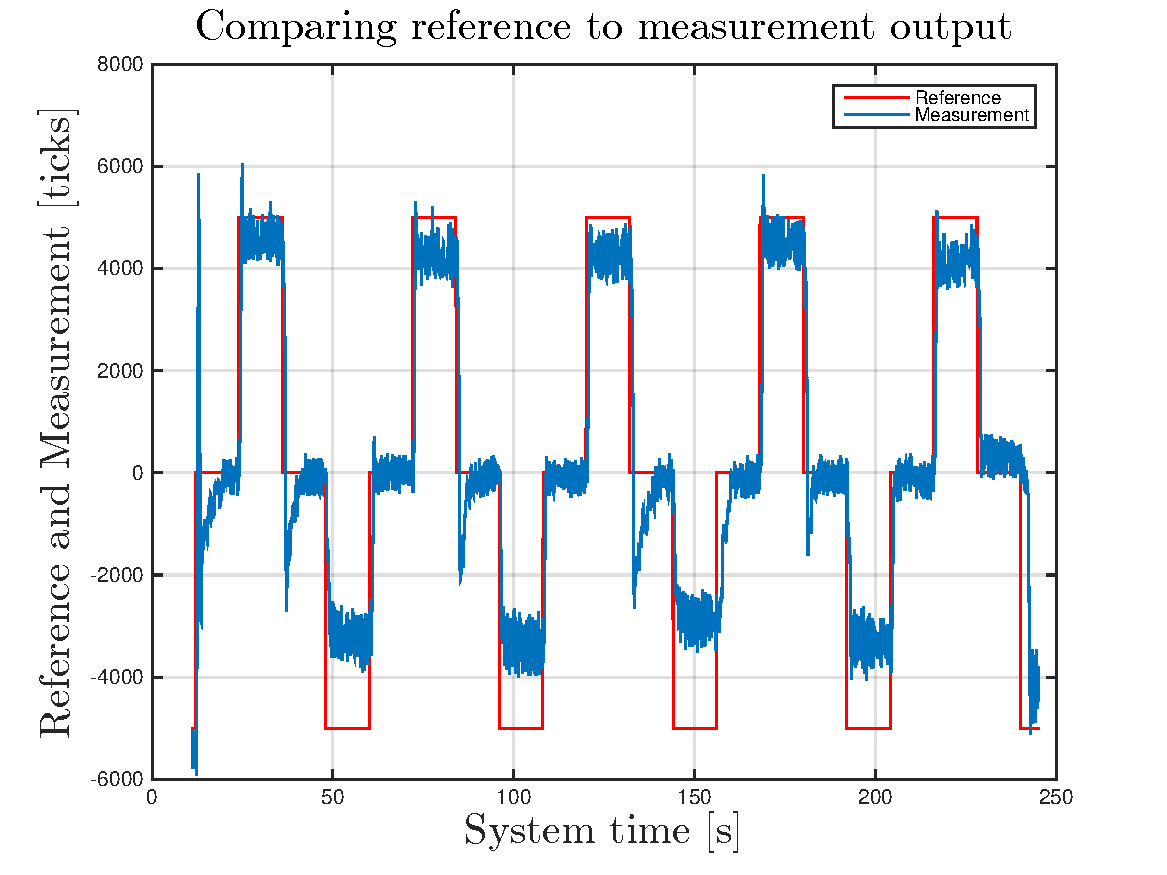
\includegraphics[width=.95\linewidth]{figures/seesaw_measurement_task2_fig1}
\caption[Measure1]{\label{f:measure1} Figure depicting the outcome of the step response task. The reference trajectory is plotted in red, while the obtained measurements are colored in blue.}
\label{fig:seesaw_task2_fig1}
\end{figure}

\begin{figure}[ht]
\centering
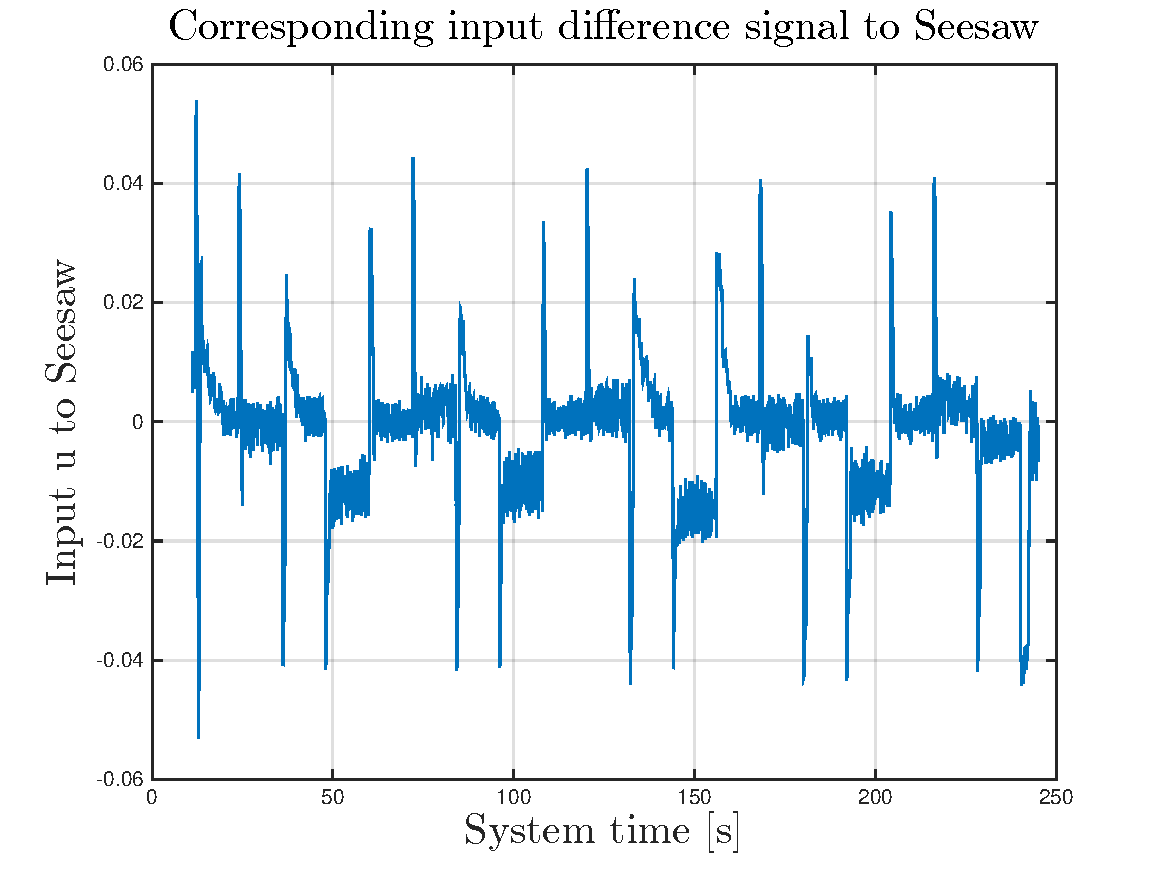
\includegraphics[width=.95\linewidth]{figures/seesaw_measurement_task2_fig2}
\caption[Measure1]{\label{f:measure1} Figure depicting the input command to the Seesaw for the step response task in blue.}
\label{fig:seesaw_task2_fig2}
\end{figure}


\begin{align*}
\text{Error}_{\text{Task 2}} &= \text{FILL IN HERE} \\
M_p & = \text{FILL IN HERE} \\
T_{90} &= \text{FILL IN HERE} 
\end{align*}

\section*{Task 3: PID with anti-reset windup}
\label{s:task_3}


\begin{enumerate}[label=\alph*)]
\item Lorem ipsum dolor sit amet, consectetur adipiscing elit, sed do eiusmod tempor incididunt ut labore et dolore magna aliqua. Ut enim ad minim veniam, quis nostrud exercitation ullamco laboris nisi ut aliquip ex ea commodo consequat. 

\item Duis aute irure dolor in reprehenderit in voluptate velit esse cillum dolore eu fugiat nulla pariatur. Excepteur sint occaecat cupidatat non proident, sunt in culpa qui officia deserunt mollit anim id est laborum.

\item -
\end{enumerate}



\begin{figure}[ht]
\centering
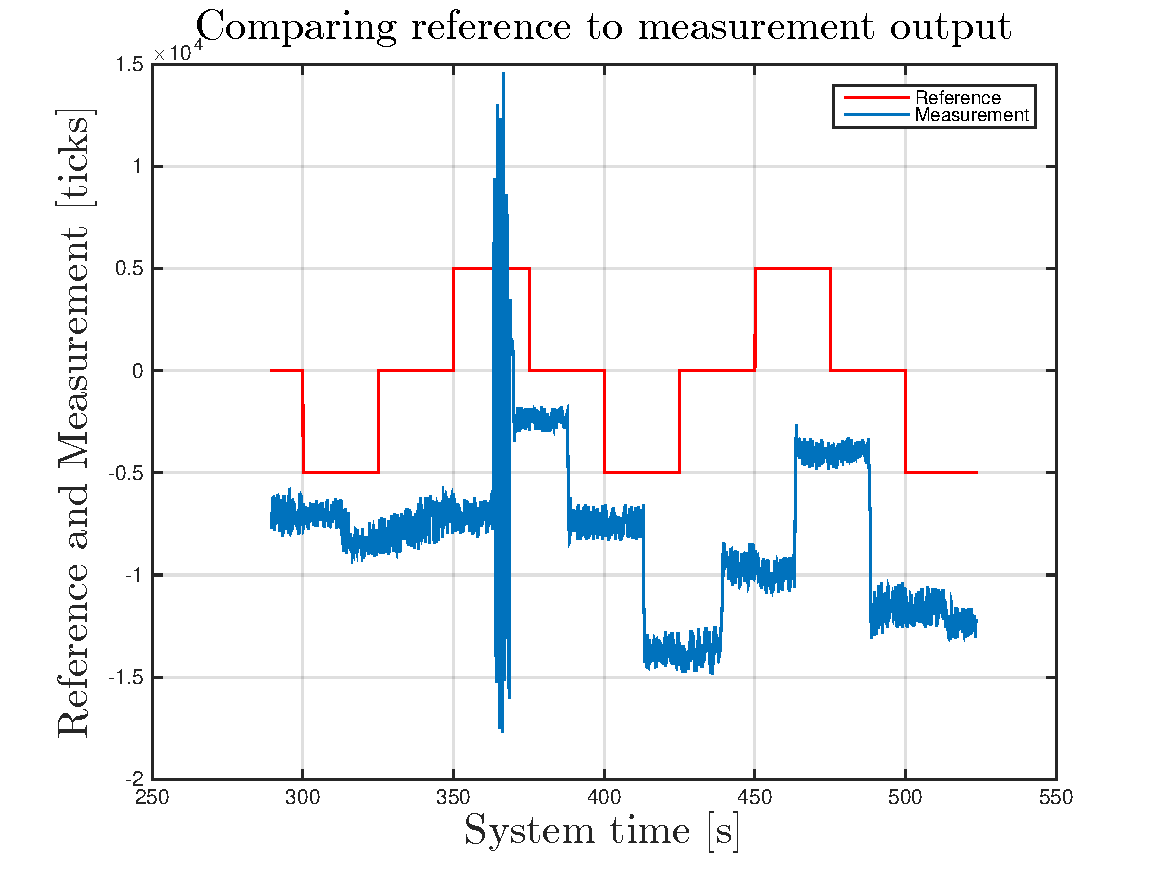
\includegraphics[width=.95\linewidth]{figures/seesaw_measurement_task3_no_ARW_fig1}
\caption[Measure1]{\label{f:measure1} Measurement and reference during prolonged integration of errors \textbf{without} anti-reset windup (ARW) scheme.}
\label{fig:seesaw_measurement_task3_no_ARW_fig1}
\end{figure}


\begin{figure}[ht]
\centering
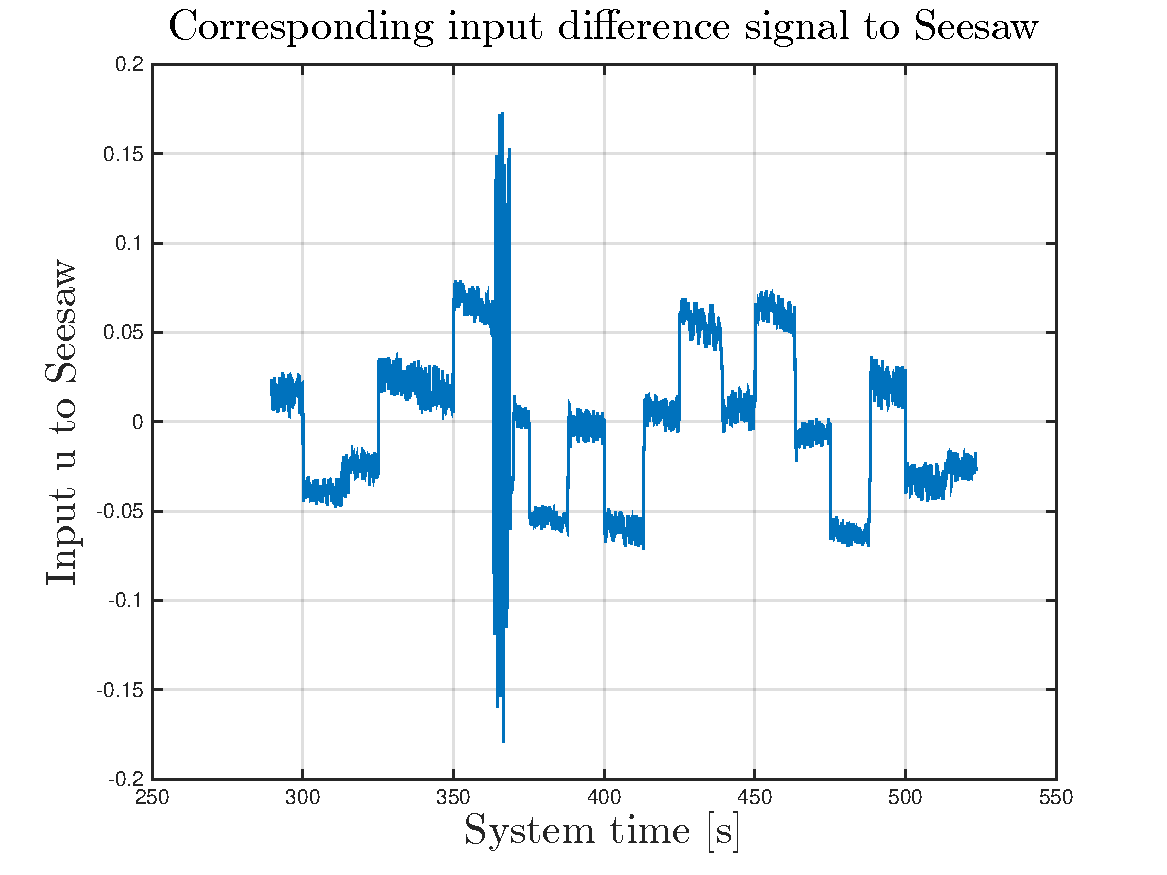
\includegraphics[width=.95\linewidth]{figures/seesaw_measurement_task3_no_ARW_fig2}
\caption[Measure1]{\label{f:measure1} Input commands during prolonged integration of errors \textbf{without} anti-reset windup (ARW) scheme.}
\label{fig:seesaw_measurement_task3_no_ARW_fig2}
\end{figure}

\begin{figure}[ht]
\centering
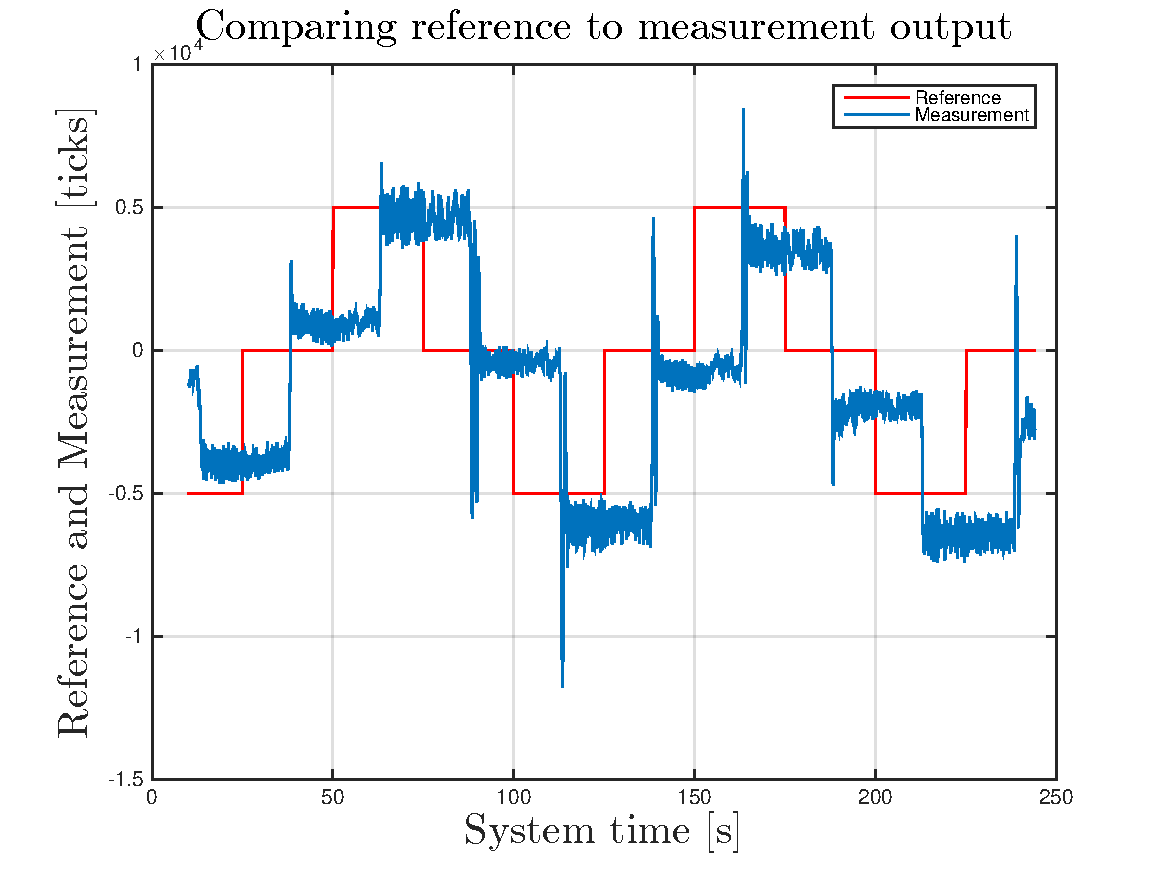
\includegraphics[width=.95\linewidth]{figures/seesaw_measurement_task3_ARW_fig1}
\caption[Measure1]{\label{f:measure1} Measurement and reference during prolonged integration of errors \textbf{with} anti-reset windup (ARW) scheme.}
\label{fig:seesaw_measurement_task3_ARW_fig1}
\end{figure}

\begin{figure}[ht]
\centering
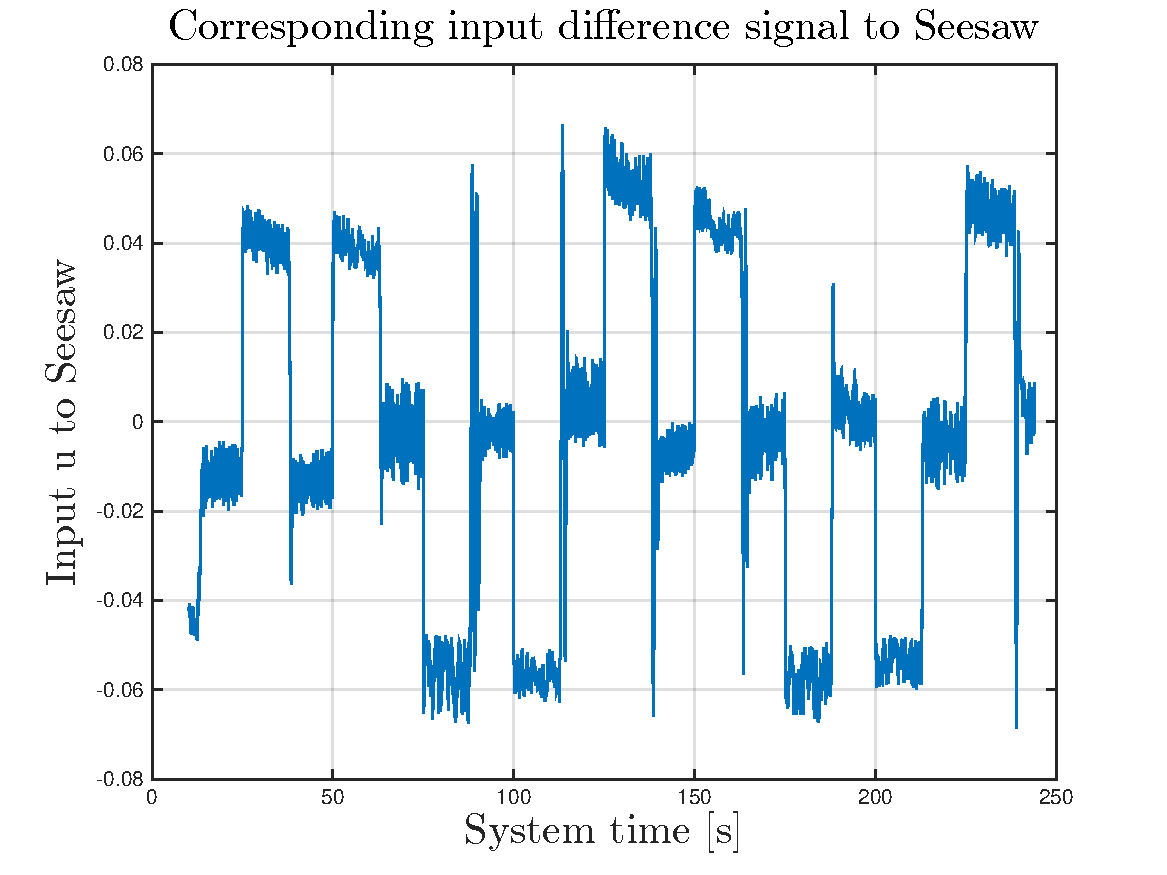
\includegraphics[width=.95\linewidth]{figures/seesaw_measurement_task3_ARW_fig2}
\caption[Measure1]{\label{f:measure1} Input commands during prolonged integration of errors \textbf{with} anti-reset windup (ARW) scheme.}
\label{fig:seesaw_measurement_task3_ARW_fig2}
\end{figure}






\end{document}
